\documentclass{standalone}
\begin{document}
\chapter{Pipeline}
The aim of this project is to implement an automated pipeline based on automatic segmentation of T2 weighted Magnetic Resonance (MR) images exploiting Convolutional Neural Networks in order to predict the response to neoadjuvant chemo-radiotherapy of colorectal cancer by using radiomic features.
\begin{figure}[htp]

    \centering
    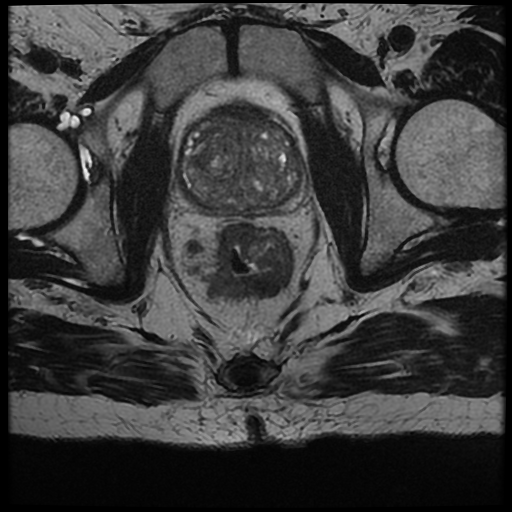
\includegraphics[width=.49\textwidth]{../images/11.png}
    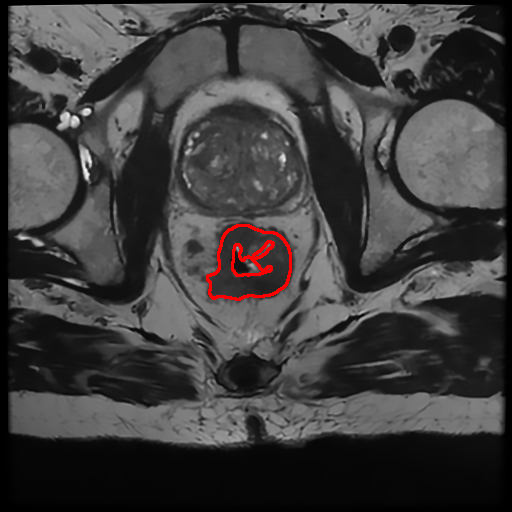
\includegraphics[width=.49\textwidth]{../images/11_cont.png}
    
    \caption{ \textit{ Left)} Original MR image of a patient affected by colorectal cancer.\textit{ Right)} The same image with identified tumor area.}
    \label{comparison}
    
    \end{figure}
    \\
The starting point is the MRI scans. 
Firstly, I started with the visualization and the pre-processing of the scans.
The pre-processing techniques consists of a smoothing filter to remove noise which could be a potential source of false positives and gamma correction to increase the brightness of the images.
The work was then split into two main frameworks: \textit{segmentation} and \textit{radiomics}.
The basic idea was to train a Convolutional Neural Network like U-Net, for the segmentation of the images.
The training process was supervised.
The input images consisted of the MRI scans and the medical annotation as ground-truth images.
Once trained the CNN model and segmented the images to obtain the colorectal cancer region, the next step was the extraction of the radiomic features.
For each patient's examination in the dataset, I extracted 100 radiomic features.
The features were then analyzed to implement a predictive model to obtain the prediction of response.
The prediction is based on the Tumor Regression Grading (TRG), which gives an evaluation of how much the chemo-radiotherapy was effective.
The workflow of the developed pipeline can be seen in Figure \ref{workflow}
\begin{figure}[htp]

    \centering
    \includegraphics[width=\textwidth]{../images/workflow2.png}
    
    \caption{Workflow of the developed pipeline. The starting point is the MRI scans. Then, the images were pre-processed for the training of a Convolutional Neural Network model. After the segmentation of the images, radiomic features were extracted from the images. They were analyzed to implement a predictive model to obtain the prediction of response based on the Tumor Regression Grade (TRG).}
    \label{workflow}
    
    \end{figure}
    \\
Obviously, the final pipeline structure does not involve a learning process and a feature analysis step since the models are already obtained.
As consequence, the final structure of the pipeline looks like in the following Figure \ref{pipeline}
\begin{figure}[ht]

    \centering
    \includegraphics[width=\textwidth]{../images/pipeline2.png}
    
    \caption{Final pipeline structure. From left to right. The MRI scans are pre-processed with a smoothing filter to remove noise and with a gamma correction to increase the brightness. Then, the segmentation is achieved by the trained CNN model. After the segmentation, radiomic features are extracted. Finally, the prediction is obtained by the implemented predictive model.}
    \label{pipeline}
    
    \end{figure}

\end{document}